\chapter{How to install and run RealTimeIoTGraph.py}
\label{How to install and run RealTimeIoTGraph.py}
%\lstinputlisting[language=Python]{appendices/sniff.py}
This chapter discusses how to install, run, and use the database visualization tool.

\section{How To Install and Run}
To install and run this analysis tool, follow the instructions at the GitHub site:   \href{https://github.com/nealhnguyen/RealTimeIoTGrapher}{github.com/nealhnguyen/realtimeiotgrapher}.

First, pull the code for this tool from git hub and install the dependencies in the requirements file through pip. At this point, the dependencies are set to run this code on python 2.7.

Next, a 'loginCredentials' file must be created containing the host, user, password, and database information. At which point, running 'python realTimeIoTGraph.py' starts the backend and display its current operation onto the terminal.

The link to the local IP address contains the graphing tool. Clicking on that opens it onto the default browser for the computer.

\section{Usage Directions}
Once the software is running, the grapher can be viewed on a web browser as shown in figure \ref{fig:grapherUsage}. This section describes each numbered element in the image.

\begin{figure}[H]
    \centering
    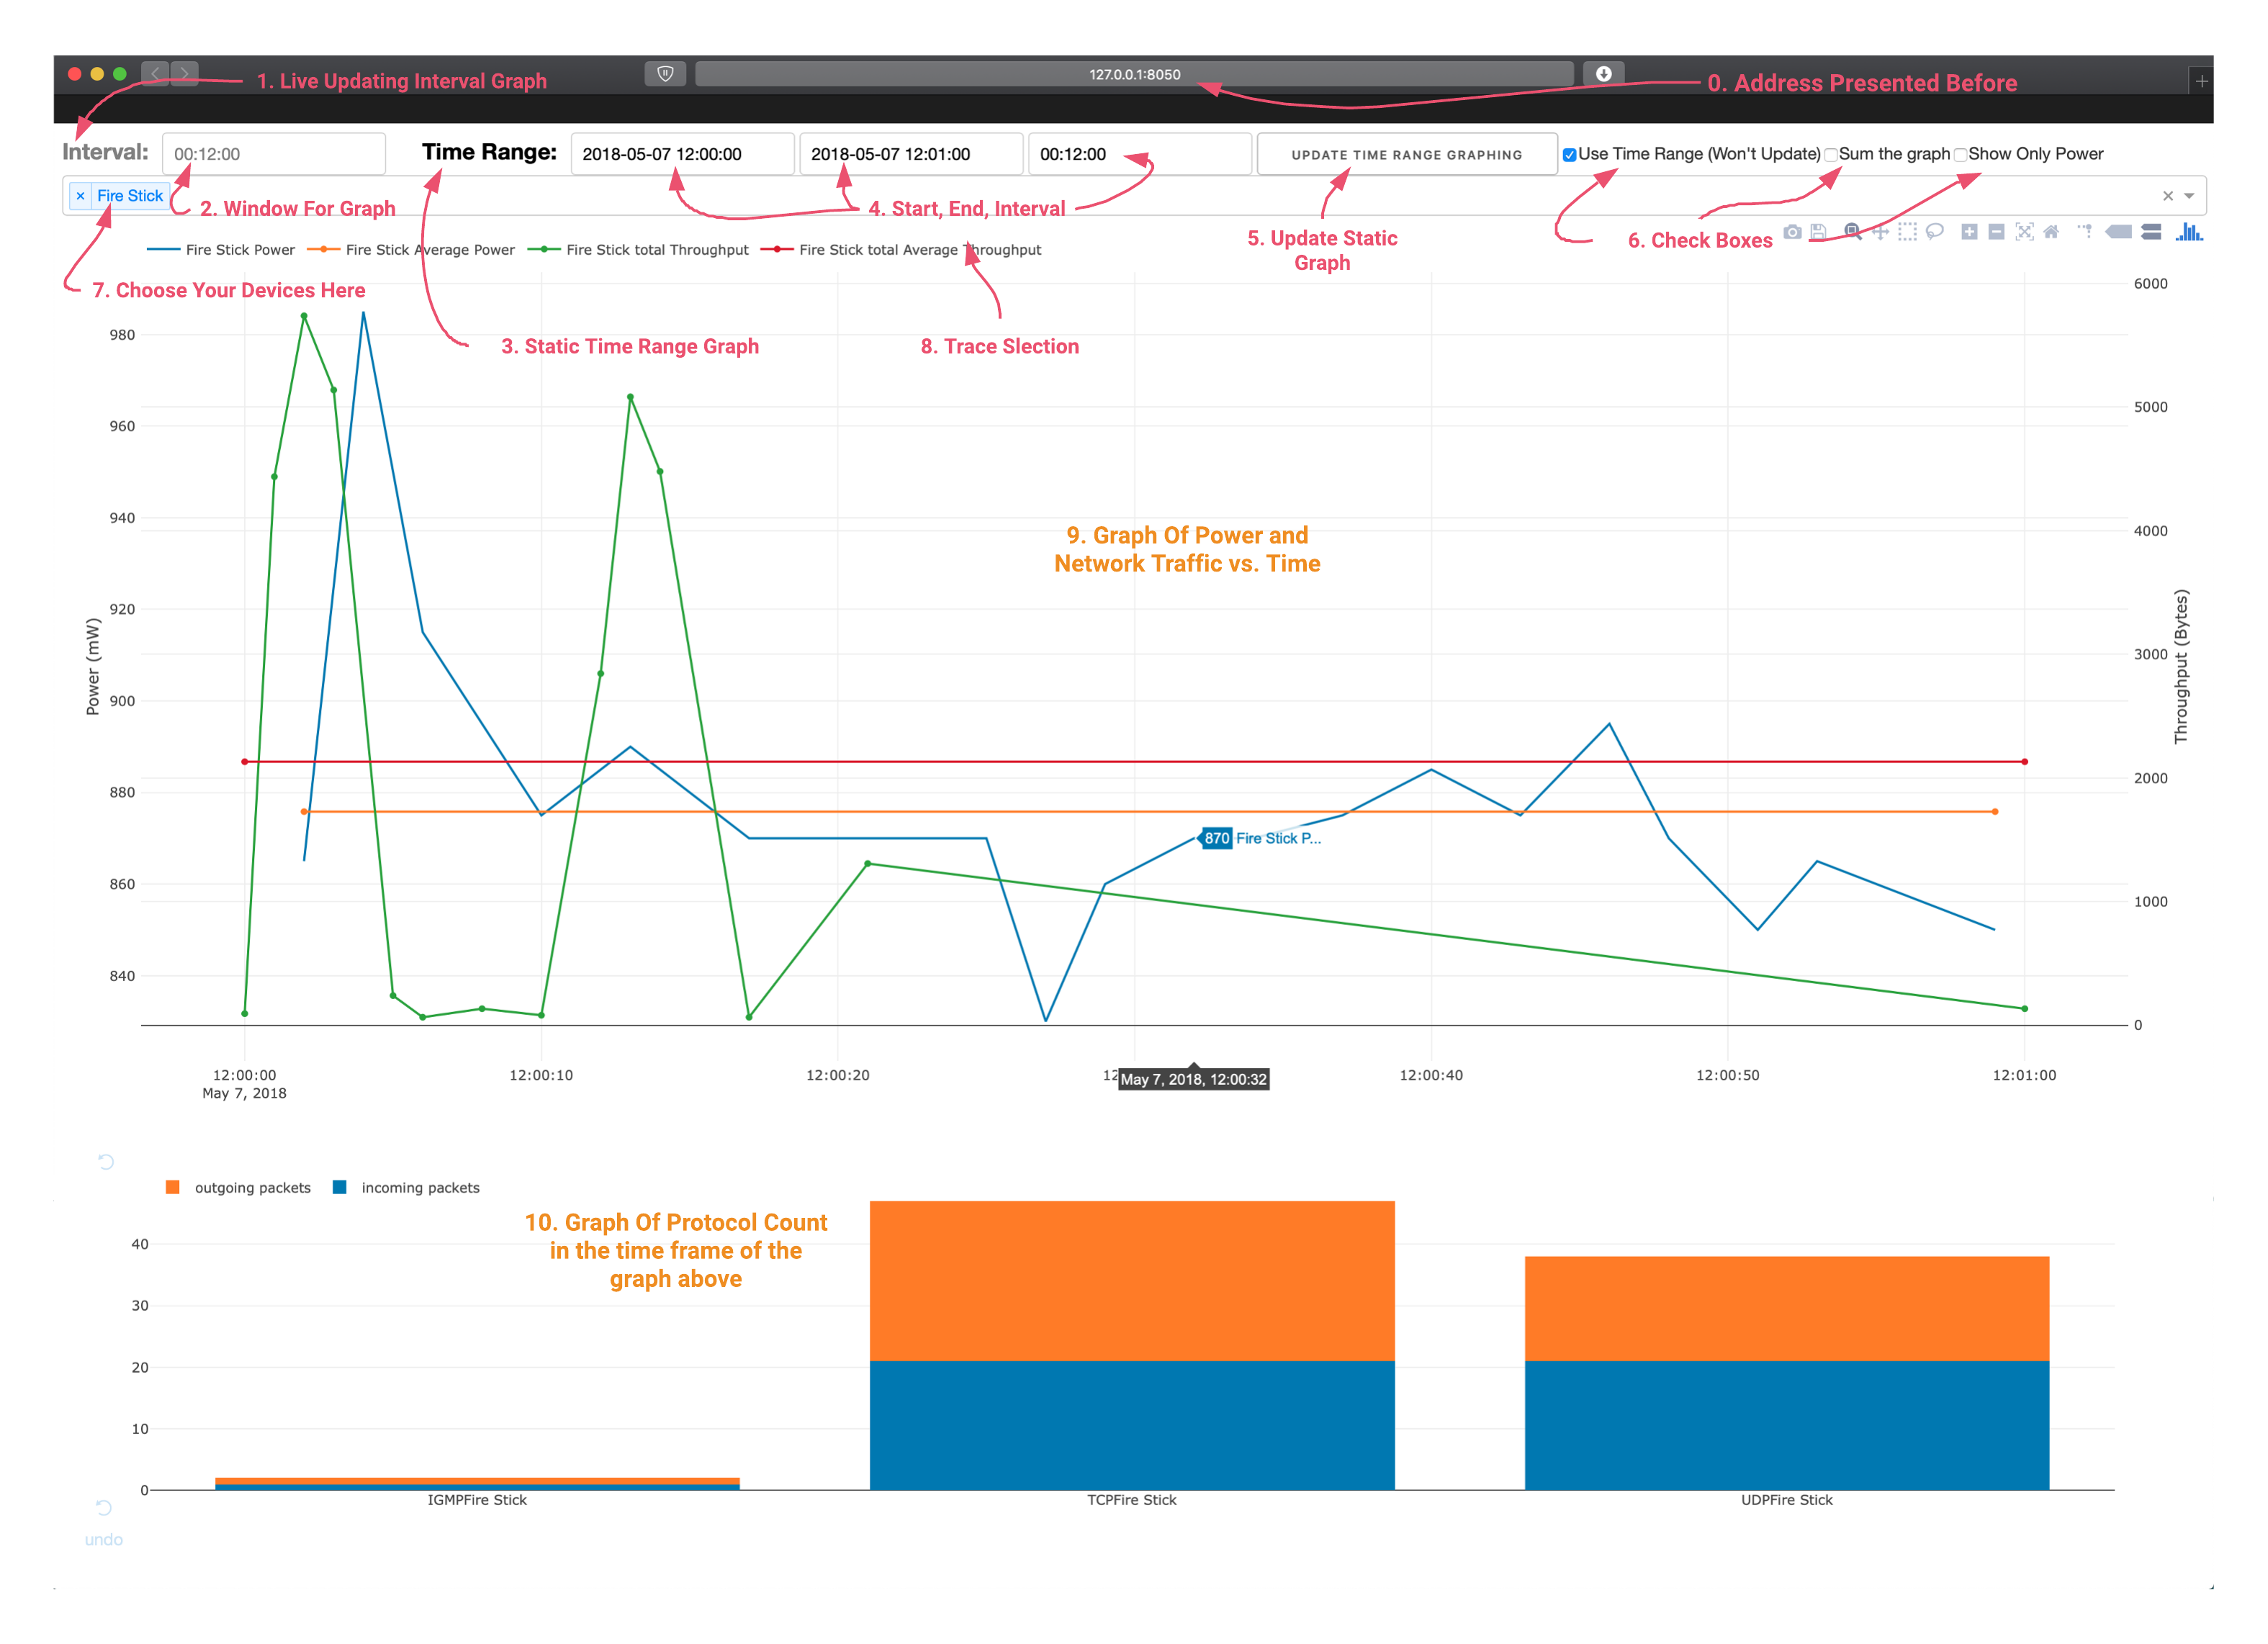
\includegraphics[width=1\textwidth]{figures/grapherUsage.png}
    \caption{RealTimeIoTGrapher usage image}
    \label{fig:grapherUsage}
\end{figure}

0. The local IP address presented in the terminal where the grapher is hosted.

1. The interval field and the text box next to it is dark when the software is in live update mode.

2. The text box here relates to the live update feature of the graph. This is a time field, denoting the window of time the graph displays at a time while it updates. The format is HH:MM:SS where HH is the hour, MM is minutes, and SS is seconds.

3. The time range field and the four elements consecutively after it are dark instead of grey when it is in static graph mode. In this state, the graphing tool specifies the network traffic and power information in the time window specified.

4. In these three text boxes, the time window for static graphing is specified. The first box is the start time, the second box is the end time, and the last box is the interval. To specify the time range, fill in any 2 of the three text boxes, and the graphing tool infers the other number. If all three text boxes are filled, then the graphing tool uses the start and end time text box. To further explain, if the start time and interval are specified, then the window is start time $\rightarrow$ start time + interval. If the end time and interval are specified, then the time window is the end time - interval $\rightarrow$ end time.

5. This button causes the graph to update. After updating the time range in step 4, clicking this button updates the graph with the new time range.

6. The ``Use Time Range'' checkbox toggles the software between live graph mode and static mode. The ``Sum Graph'' checkbox sums up all power graphs into one. The ``Show Only Power'' checkbox allows the grapher to avoid a SQL query for the network throughput, speeding up the process in case of pure power analysis.

7. This selection field specifies all the devices the software creates graphs. One, or many devices can be specified at a time. If too many devices are specified at a time, the software may run slow.

8. The traces shown can be selected or deflected to toggle its visibility.

9. This line graph displays the number of bytes sent through the network by a device going in, out, and in total. It also shows the power usage over time. Also, it shows the average value for a graph in the interval of the graph

10. This bar graph displays the spread of network traffic by protocol for each device. It displays the outgoing packets as orange and incoming packets as blue. It displays an individual bar graph for each device and protocol. Similarly, the traces can be clicked on to hide its visibility.